\chapter{Evaluation} \label{evaluation}

\section{Metrics}
Alongside properties discussed in Sections \ref{sec: life-like-exploration} and \ref{sec: gs-exploration}, we design metrics to categorise CA and assess the effectiveness of evolutionary algorithms.

\subsection{Dynamic Metrics}
We say a dynamic metric is one that tells us about the way a CA's state changes over time. Two useful dynamic metrics are periodicity and volatility.

It is useful to know when a CA has converged to a fixed point or periodic solution. By estimating the portion of initial conditions that enter a periodic state, and the speed with which they do so, we can infer the Wolfram class of CAs with reasonable accuracy. The key distinction we intend to make here is between CAs in class 1 or 2 against CAs in class 3 or 4. The former two classes should converge relatively quickly for almost all ICs whereas the latter two will not converge for a significant proportion of ICs.

\begin{definition}[CA convergence to a periodic state]
 If a state previously visited at time step $t$ is produced again at step $t+\delta$, the rule is said to have converged to a periodic solution at $t+\delta$ time steps with period $\delta$. If $\delta = 1$, this is called a fixed point solution. 
\end{definition}

For the trivial initial conditions with all zero-cells or all one-cells, all life-like CAs will converge to a periodic state with $\delta \leq 2$. The proof of this is detailed in \ref{quiescent-nullity}.

\begin{definition}[Quiescence]
A CA is quiescent if all cells are in the same state. A CA with each cell $c_i$ in state $\sigma_i(t) = 0$ is denoted $\vec{0}$ and the opposite quiescent CA with $\sigma_i(t) = 1$ is denoted $\vec{1}$. 
\end{definition}

\begin{lemma}
A quiescent life-like CA is at a fixed point or oscillates with period 2.   
\end{lemma}

\begin{proof} \label{quiescent-nullity}
Consider an arbitrary cell $c_i$ in $\vec{0}$. $\sigma_i(t)$ is the state of $c_i$ at time t and $n_i(t)$ is the number of live cells in the neighbourhood of $c_i$ not including itself. Initial conditions are $\sigma_i(0) = 0 \text{\ and\ } n_i(0) = 0$.
\begin{multicols}{2}
\noindent If $0 \notin B$:\\
\null \quad $\sigma_i(1) = 0 \text{\ and\ } n_i(1) = 0 $\\
\null \quad $\implies$ convergence to $\vec{0}$ with period 1.\\
\columnbreak\linebreak
\noindent If $0 \in B$:\\
\null \quad $\sigma_i(1) = 1 \text{\ and\ } n_i(1) = 8 $\\
\null \quad If $8 \in S$:\\
\null \qquad $\sigma_i(2) = 1 \text{\ and\ } n_i(1) = 8 $\\
\null \qquad $\implies$ convergence to $\vec{1}$ with period 1.\\
\null \quad If $8 \notin S$:\\
\null \qquad $\sigma_i(2) = 0 \text{\ and\ } n_i(1) = 0 $\\
\null \qquad $\implies$ oscillation between $\vec{0}$ and $\vec{1}$.
\end{multicols}
\noindent The case for a CA at quiescent state $\vec{1}$ is exactly symmetrical.
\end{proof}

\todo{Def of volatility?}

Another useful measure is volatility, which measures the average number of cells that change per time step. We expect class 1 CA to have a volatility that approaches zero. Class 2 and 3 CA will have a volatility that approaches a non-zero constant. Class 4 CA can have a volatility that does not converge at all.\\

\subsection{Static Metrics} 

\todo{Def of density?}
A static metric is one that assesses the state of the CA at one snapshot in time, ideally after some fixed number of time steps $t$.
A good way to separate class 1 and class 2 CA is to observe their density at $t$ time steps. Density is the average number of live cells in the CA state. If the CAs have converged to their respective cycles, we will find that class 1 CA have density of 0 or 1 for almost all initial conditions whereas class 2 CA will regularly have densities that are in between 0 and 1.\\

\todo{Entropy metric??}
% \subsection{Entropy}
% By making repeated observations on the state of the CA after a set number of time steps, say $t$, we can assess average the amount of "information" in the state at time $t$. This helps us differentiate class 3 CAs which enter a state of unending chaos after transient patterns have dissolved. Information entropy is a useful measure of this information.
% \begin{definition}[Entropy] Consider a CA with state $X$ at time $t$. We define the entropy of the CA at this point as
    
% \end{definition}

% %COMMENT
% % The problem here is that IC ~ binomial which is approx normal for p =0.5 but only using ICs with p=0.5 unfairly advantages CAs with birth or survival rates around 4. But if we use ICs uniform across density then the binomial = normal assumption breaks.

\subsection{Similarity}

It is useful to evaluate the manner in which a population converges towards solutions during evolution. Although we reuse the word convergence to describe this, note the difference between a CA converging to a periodic solution and a population converging towards an optimal transition function. To evaluate the convergence of a population, it is useful to have a notion of similarity between individuals. This allows us to quantify the speed of convergence and group individuals into families if they are converging towards different optima. For a binary string chromosome, the simple matching coefficient (SMC) between two individuals is an appropriate metric to quantify their relative similarity. 
\begin{definition}[Simple Matching Coefficient] Consider two binary strings $A$ and $B$. The frequency table enumerating the number of instances of each possible combination of bit settings is
\begin{center}
    \begin{tabular}{ c c c }
              & $A_i = 0$ & $A_i = 1$ \\ 
        $B_i = 0$ & $n_{0,0}$ & $n_{1,0}$ \\  
        $B_i = 1$ & $n_{0,1}$ & $n_{1, 1}$    
    \end{tabular}
\end{center}
The simple matching coefficient between two binary strings $A$ and $B$ of length $n$ is\\
\[
    SMC = \frac{n_{0, 0} + n_{1, 1}}{n_{0, 0} + n_{1, 1} + n_{0, 1} + n_{1, 0}}
\]
    
\end{definition}
Symmetrically, we consider the Simple Matching Distance, $\textnormal{SMD} = 1 - \textnormal{SMC}$, as a measure of diversity between individuals. This is appropriate as SMD fulfills all the formal criteria for a distance metric: non-negativity, symmetry, identity of indiscernibles, and the triangle inequality. If each bit is to be imagined as a gene, the SMD is the mean number of differing genes in the chromosome. It can be calculated in $O(n)$ time where $n$ is the chromosome length. Aside from being simple to understand and efficient to calculate, the SMD is preferable to other metrics as it accounts for mutual presence and mutual absence. Jaccard Distance $d_J$, on the other hand, only registers mutual presence. For two binary strings $A$ and $B$
\[
    d_J = \frac{n_{0, 1} + n_{1, 0}}{n_{0, 1} + n_{1, 0} + n_{1, 1}}
\]
This is useful in settings where true negatives ought to be ignored. For example, when testing if two water samples came from the same source, we would not be interested in enumerating all the compounds that are \textit{not} present in both samples. However, our use case benefits from knowing when a gene is \textit{not present} in both chromosomes as much as knowing if it \textit{is present} since both of these properties can equally affect CA dynamics. For this reason we use the Simple Matching Distance.

\section{Exploration}

When evaluating the effectiveness of evolutionary techniques at learning life-like CA rules, it is important to contextualise quantitative properties like convergence rate, fitness, and diversity. We begin by performing an exploratory statistical analysis to gather data on the life-like CA rule space. In conjunction with the analyses of Wolfram\cite{wolfram1986theory} and Eppstein\cite{eppstein2010growth}, this will shed light into the characteristics that make a rule easier or harder to predict.\\

There are $2^{18} = 262144$ possible outer-totalistic cellular automata rules which makes a systematic analysis of their properties feasible through random simulation. 100 initial conditions are sampled from a distribution uniform across densities 0 to 1. Each rule is simulated on each initial condition for 100 time steps and the state at each step is recorded in a hashmap. We examine each rule to find the percentage of initial conditions that converge within 100 steps and the mean oscillation period of those that converge.\\   

\todo{EXPERIMENT 1}: TODO - Redo this analysis with fixed simulator and newer metrics

---- OLD STUFF STARTS HERE
\begin{figure}[!h]
\centering
            \subfloat{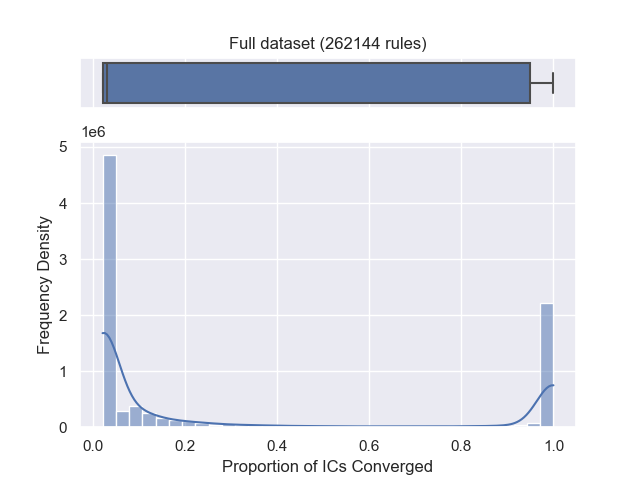
\includegraphics[width=.5\textwidth]{images/full-taxonomy.png}}\hfill
            \subfloat{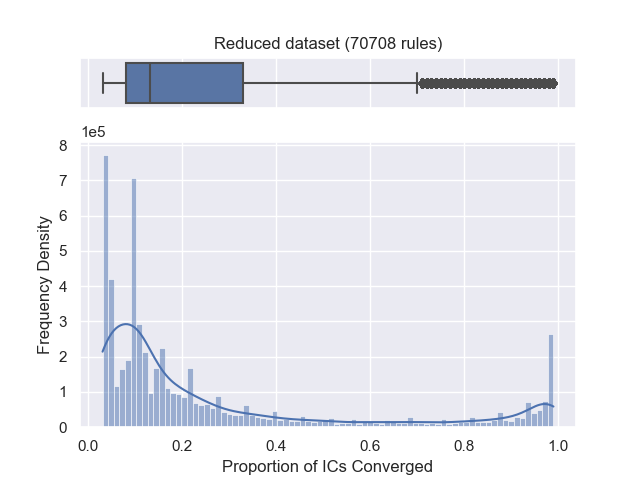
\includegraphics[width=.5\textwidth]{images/reduced-taxonomy.png}}\hfill
            \caption{Distributions of convergence of full and reduced set of life-like CAs}
\label{fig:taxonomy-dist}
\end{figure}

First we consider the two extremities. 23.2\% of rules converge for all initial conditions and 49.8\% of rules converge for only 2 out 100 initial conditions. Note this is the minimum convergence number in our setting since all rules will converge for the trivial initial conditions with density 0 and density 1.  This leaves 27.0\% or 70708 of the original rules remaining. While the original dataset had a median of 3\% convergence, the reduced set of rules present a more even spread with a median of 13\%.
---- OLD STUFF ENDS HERE

\section{Maze Generation}

We begin by evaluating the effectiveness of the maze generator at maximizing the two fitness metrics. These are the length of the solution path ($p$) and the number of dead ends ($d$). From spot checks on a few examples in the simulator, we find that these two metrics happen to have similar ranges (around 70-100). For this reason we begin by treating them with equal weighting during hyperparameter tuning.\\

\subsection{Hyperparameter Tuning}

We perform a grid search on training hyperparameters across the following ranges
\begin{center}
    \begin{tabular}{ l c }
        \bf Hyperparameter & \bf Values Tried\\
        Number of Epochs & 10, 50, 100\\
        Population Size & 20, 50, 100\\
        Elitism Rate & 0.1, 0.2, 0.5\\
        Mutation Rate & 0.01, 0.05, 0.1
    \end{tabular}
\end{center}

\begin{figure}[!h]
\centering
            \subfloat[Fitness across both metrics, $d$ against $p$.]{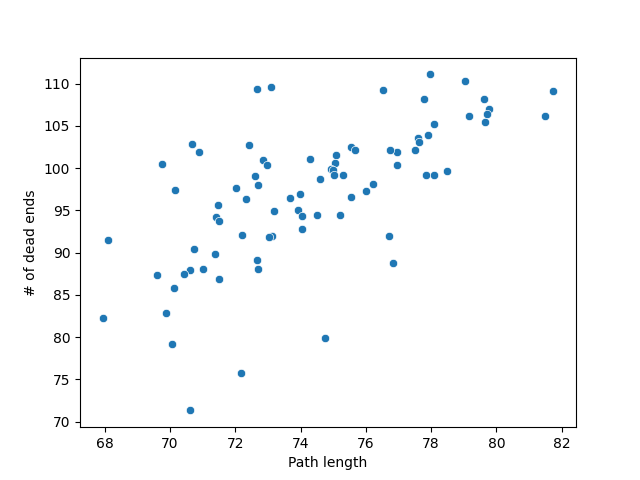
\includegraphics[width=.45\textwidth]{images/maze_hyperparam_notime.png}}\hfill
            \subfloat[Runtime adjusted fitness. $\frac{d}{t}$ against $\frac{p}{t}$ with log axes.]{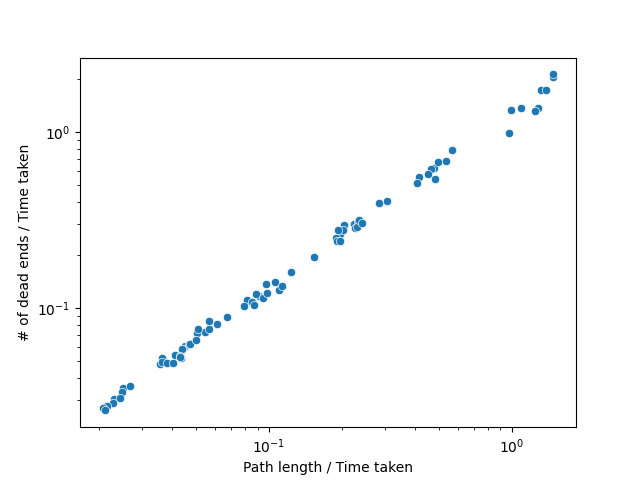
\includegraphics[width=.45\textwidth]{images/log_maze_hyperparam.png}}\hfill
            \caption{Fitness of different hyperparameter configurations across both metrics for maze generation}
\label{fig:maze-hyperparam}
\end{figure}

The optimum metrics achieved are ($d=109.1$, $p=81.8$) with configurations (number of epochs = $100$, population size = $20$, elitism rate = $0.5$, mutation rate = $0.01$). Under a time adjusted measure, we try to optimize for the value of the metric achieved relative to the execution time. Here, the optimum value is ($d=100.5$, $p=69.8$) for configurations (number of epochs = $100$, population size = $20$, elitism rate = $0.1$, mutation rate = $0.05$). This is not significantly worse than the optimum value achieved when disregarding execution time.

\subsection{Ablation Analysis}
Hyperparameter tuning revealed that the lowest mutation rate produced the best results. This suggests that mutation may not be necessary for maze evolution. To test this hypothesis, we conduct an ablation analysis on the genetic operators used. We run 10 maze generations, each for 100 epochs. We use the optimal runtime-adjusted hyperparameters for efficiency. We then repeat this procedure, each time systematically adding and removing genetic operators from the learning procedure. Figure~\ref{fig:maze-ablation} shows a kernel density estimate plot which visualises the area occupied by the optimal results produced by each of these learning procedures.\\

\begin{figure}[!h]
\centering
            \subfloat[Mutation and no crossover]{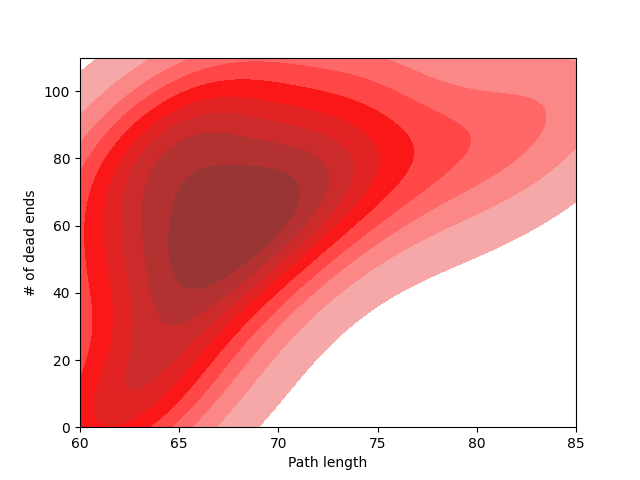
\includegraphics[width=.3\textwidth]{images/maze_eval/cross-kde.png}}\hfill
            \subfloat[Crossover and no mutation]{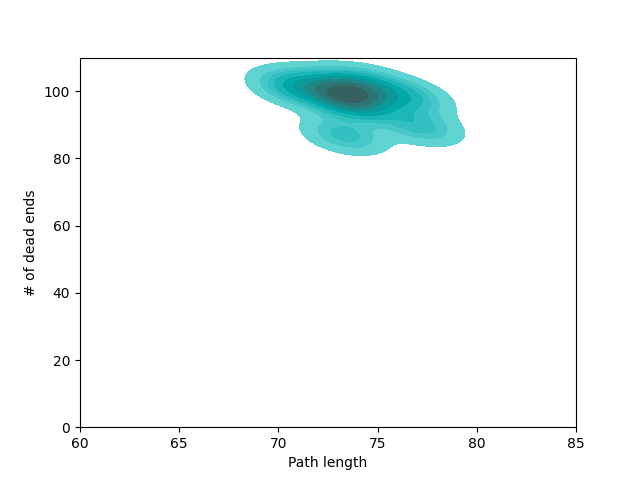
\includegraphics[width=.3\textwidth]{images/maze_eval/mutation-kde.png}}\hfill
            \subfloat[Both mutation and crossover]{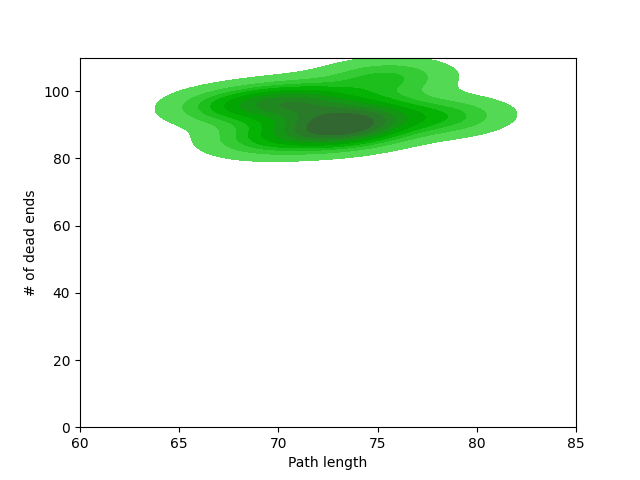
\includegraphics[width=.3\textwidth]{images/maze_eval/both-kde.png}}\hfill
            \caption{Optimum results produced when removing mutation and crossover components for mazes}
\label{fig:maze-ablation}
\end{figure}

It is clear that crossover is important for convergence to a strong solution as the experiment without crossover had a much higher variance in the results produced. However, mutation appears to have a much smaller effect in this case. Without mutation, we obtain a slightly higher variance in results produced and these results tend to have a lower number of dead ends. If both mutation and crossover are omitted, no learning occurs and we find no legitimate mazes in the majority of cases.

\subsection{Objective vs Relative Fitness}

Since we are optimising for two metrics, we can take a linear combination of the objective values of $p$ and $d$ or we can rank each candidate separately by $p$ and $d$ then take a linear combination of the ranks. We call this objective and relative fitness respectively. For each fitness type, we run 20 experiments with a bias of 0.5 (i.e. equal weighting to the two goals) In Figure~\ref{fig:objective} KDE plots show the difference in performance of roulette and truncation selection using each of objective and relative fitness for selection. Note that the x axis here is still objective fitness as that is what the algorithm as a whole is attempting to maximise.\\

\begin{figure}[!h]
\centering
            \subfloat[Objective Fitness]{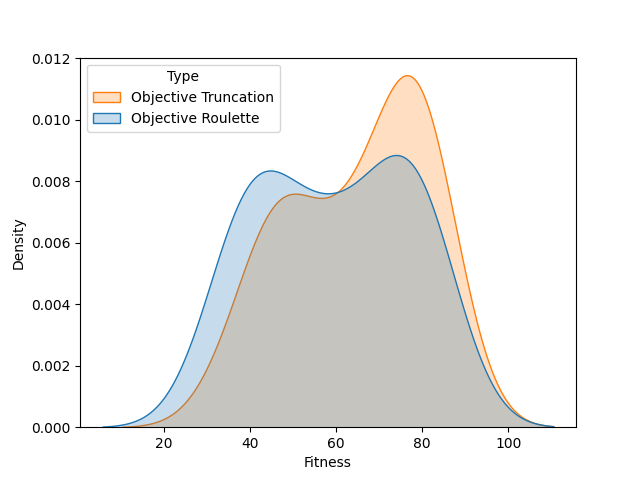
\includegraphics[width=.5\textwidth]{images/objective-fitness.png}}\hfill
            \subfloat[Relative Fitness]{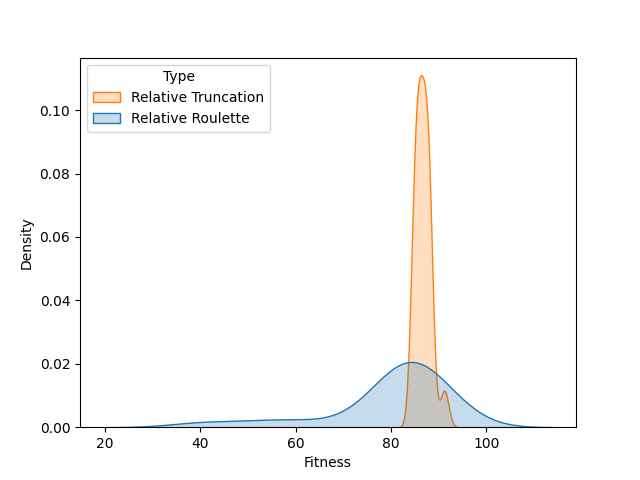
\includegraphics[width=.5\textwidth]{images/relative-fitness.png}}\hfill
            \caption{Objective and relative fitness for roulette and truncation selection}
\label{fig:objective}
\end{figure}

Under both objective and relative fitness, truncation selection outperforms roulette selection on average. There is also a lower variance in the fitness of solutions produced using truncation selection. This is especially exemplified in the case with relative fitness. One reason for this is the decreasing variability in fitness of elite candidates as the population evolves. This makes a roulette selection increasingly likely to pick suboptimal parents. Truncation selection, on the other hand, asserts that a selected candidate will never have a lower fitness than a candidate that has not been selected. However, this can also increase the likelihood of premature convergence since genes within incrementally worse solutions that have potential to produce global optima are lost. Based on the results shown, we opt for a truncation selection using relative fitness. It is interesting to see that a alternative selection criterion, relative fitness, can optimize the objective function better than using the objective function itself for selection.

\subsection{Bias Tuning}
The bias parameter $\lambda$ decides the weighting given to solution path length over number of dead ends when calculating fitness. Although this can be set by the user based on personal preference, we can tune the bias to find the value that maximizes overall fitness  $f(\lambda) = \lambda \hat{p}_\lambda + (1-\lambda)\hat{d}_\lambda$ where $ \hat{p}_\lambda$ and $\hat{d}_\lambda$ are the optimal values discovered by the algorithm under a bias of $\lambda$.\\ 
\begin{figure}[!h]
\centering
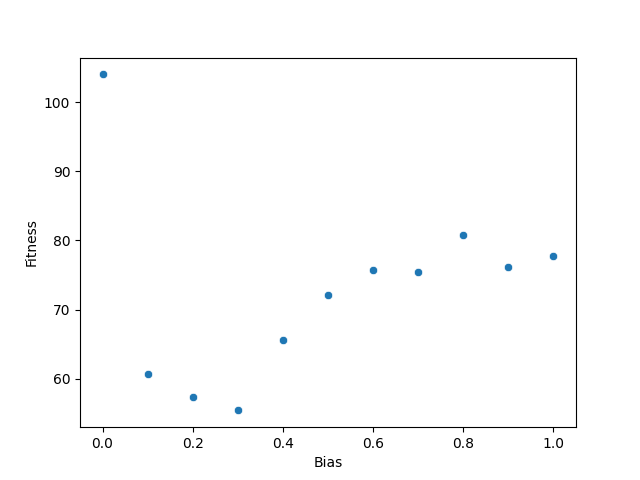
\includegraphics[width=0.7\textwidth]{images/bias-tuning.png}
\caption{Best fitness rule strings discovered under different bias values $\lambda$}
\label{fig:bias-tuning}
\end{figure}
Figure~\ref{fig:bias-tuning} shows that the algorithm performs best for higher bias values except $\lambda=0.0$ which has a very high performance. For a maze with a mix of dead ends and long solution path, the user may find better results from a bias of around 0.5 than around 0.3. Figure~\ref{fig:bias-mazes} shows the top mazes produced for different bias values. Qualitatively these appear to optimize the metrics they are being tested against.\\
\begin{figure}[!h]
\centering
            \subfloat[B16/S1235 ($\lambda=0.0$)]{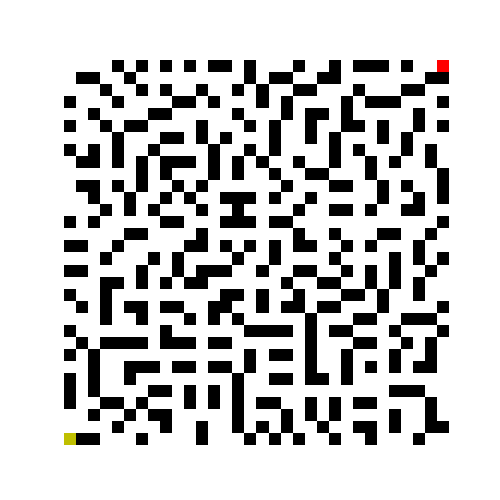
\includegraphics[width=.33\textwidth]{images/0-bias-maze.png}}\hfill
            \subfloat[B2678/S12348 ($\lambda=0.4$)]{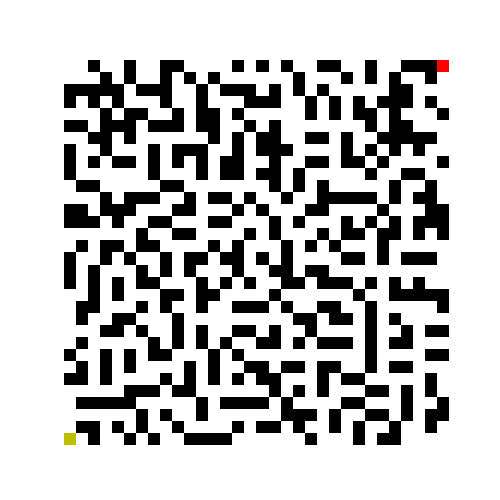
\includegraphics[width=.33\textwidth]{images/40-bias-maze.png}}\hfill
            \subfloat[B238/S12356 ($\lambda = 1.0$)]{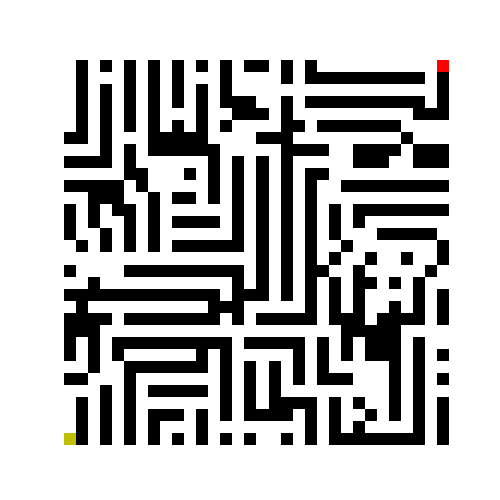
\includegraphics[width=.33\textwidth]{images/100-bias-maze.png}}\hfill
            \caption{Best mazes produced from rules discovered using different bias values}
\label{fig:bias-mazes}
\end{figure}

\section{Life-Like CA}

\subsection{Single Case Evaluation} \label{sub:single-case}

We begin by attempting to learn for a few specific rules to test the efficacy of the learning process. Consider Conway's Life rule B3/S23. In binary this is '000100000001100000' and as an integer it is 16480. Based on spot checks, we use the following hyperparameters\\ 
\begin{center}
    \begin{tabular}{ l c }
        Number of Epochs & 30\\
        Population Size & 20\\
        Number of Initial Conditions & 20\\
        Elitism Rate & 0.2\\
        Mutation Rate & 0.05\\
        Evaluation Steps & 10\\
        Minimum Step Size & 1\\
        Maximum Step Size & 5\\
    \end{tabular}
\end{center}
These have been obtained by looking at common parameters used in the literature\todo{cite}, using parameters from the maze generation experiments, and running spot checks on a few examples. A more rigorous hyperparameter tuning of the final 3 parameters is covered in Subsection~\ref{sub:stepsize}. We test on initial conditions sampled uniformly on density.\\ 

\begin{figure}[!h]
\centering
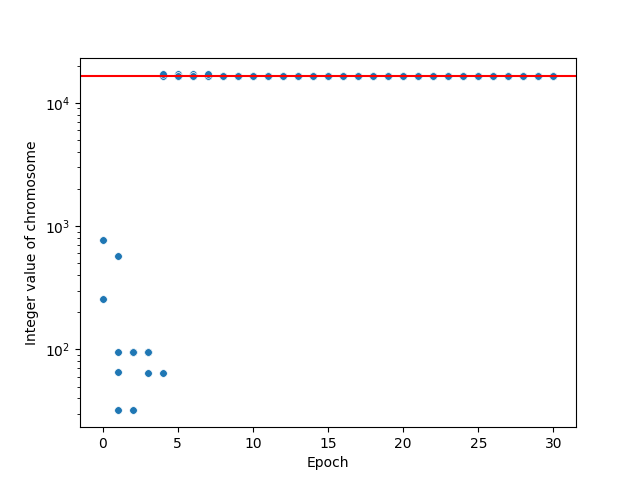
\includegraphics[width=0.7\textwidth]{images/life_like_eval/life-convgraph.png}
\caption{Top 4 elite rules from each epoch in an experiment learning Life. The red line represents the goal.}
\label{fig:life-convgraph}
\end{figure}

Figure~\ref{fig:life-convgraph} shows the algorithm to be very successful at learning the Life rule. In this experiment, the algorithm converges to the correct solution in 5 epochs. At many epochs, and especially after the true rule has been discovered, we see less than 4 points because a few of the elite rules are the same. Note that the graph has a log y-axis, so convergence is extremely fast.\\

\begin{figure}[!h]
\centering
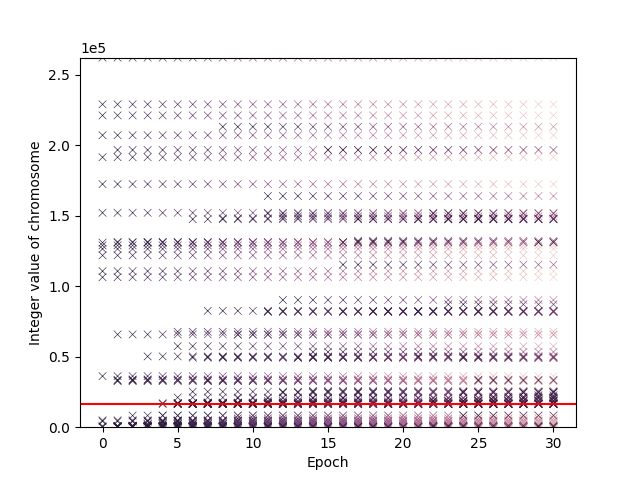
\includegraphics[width=0.7\textwidth]{images/life_like_eval/life-searchgraph.png}
\caption{All visited rules during evolution. Each rule is represented as a dark cross when first discovered and gradually fades in colour from left-to-right. The red line represents the goal.}
\label{fig:life-searchgraph}
\end{figure}

Figure~\ref{fig:life-searchgraph} shows the portion of the search space visited by the algorithm. As we can see, the top areas far from the goal quickly fade away as selection pressure removes such solutions and offspring in this area are no longer produced. We can also see some other dark bands existing far from the goal at epoch 30. The evolution history shows that by epoch 8, all the elite candidates are identical copies of the goal. This means that the dark bands seen at the end of the graph are not local optima but rather instances of the limited types of offspring that can be produced by applying crossover between two identical rule strings representing the goal solution.

\subsection{Ablation Analysis}
Ablation analysis reveals that both mutation and crossover are critical to achieving a performance like this. Consider Figure~\ref{fig:life-ablation}. 'Visited' indicates the number of unique candidates considered by the algorithm in 30 epochs. Under no mutation and no crossover, we see that the population does not evolve at all. The number of visited candidates is equal to the initial population size, 20. With mutation but no crossover, the algorithm is incapable of convergence as it is unable to retain generational knowledge. With crossover but no mutation, the algorithm quickly converges to a local minimum from which it is powerless to escape. This also stagnates the number of candidates visited to 37. When both mutation and crossover are maintained, the algorithm successfully converges to the global minimum.\\ 

\begin{figure}[!h]
\centering
            \subfloat[No mutation and no crossover (visited = 20)]{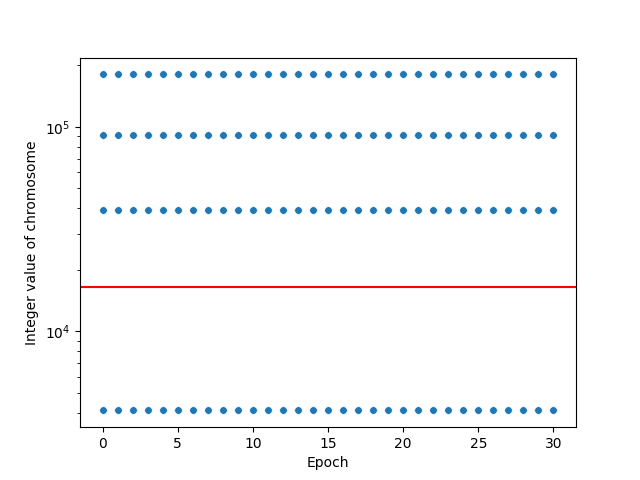
\includegraphics[width=.5\textwidth]{images/life_like_eval/life-nothing.png}}\hfill
            \subfloat[Mutation and no crossover (visited = 90)]{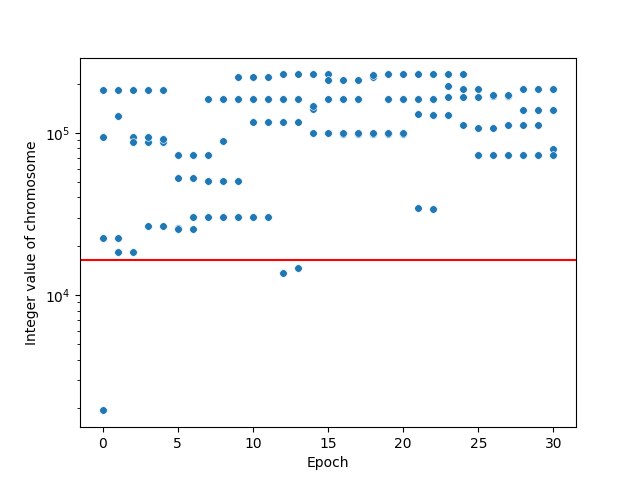
\includegraphics[width=.5\textwidth]{images/life_like_eval/life-no-crossover.png}}\hfill
            \newline
            \subfloat[Crossover and no mutation (visited = 37)]{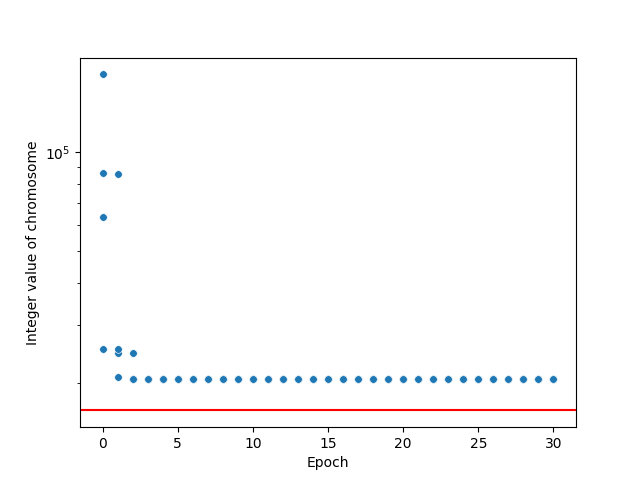
\includegraphics[width=.5\textwidth]{images/life_like_eval/life-no-mutation.png}}\hfill
            \subfloat[Both mutation and crossover (visited = 197)]{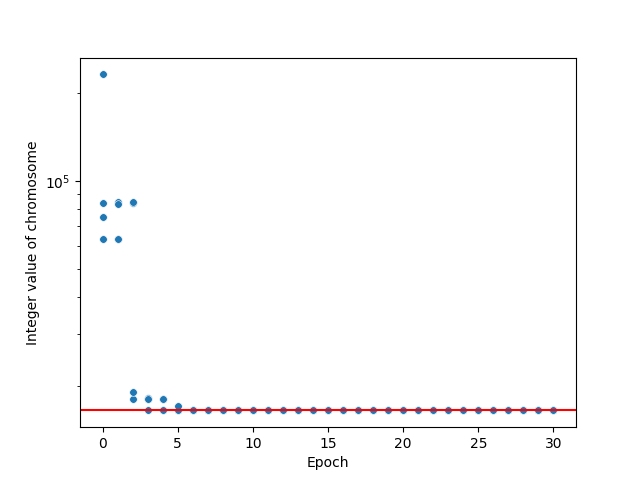
\includegraphics[width=.5\textwidth]{images/life_like_eval/life-both.png}}\hfill
            \caption{Optimum results produced when removing mutation and crossover components for modelling life-like CA}
\label{fig:life-ablation}
\end{figure}

\subsection{Stepsize Tuning}\label{sub:hyperparameter-tuning}
 
Since the rule space is of order $10^6$, performing hyperparameter tuning across all parameters on a representative sample of the search space would be infeasible in the given time frame with the resources available. We find the parameters established in \ref{sub:single-case} to be appropriate based on spot checks on a set of rules covering all 4 Wolfram classes. These bear some similarity to the hyperparameters established in the procedural generation case. One point of interest is optimising the number of evaluations and the stepsize as these factors have considerable effect on the training time.\\

Considering a random uniform stepsize, $\delta_k \sim \mathit{Uniform}(D_{max}, D_{min})$ we set $D_{min} = 1$ since we would like to give the algorithm a chance of learning on very small steps. To determine $D_{max}$, the algorithm is run on 100 goal rules sampled uniformly across the integer rule values and each the loss of each rule is calculated by simulating on 20 random initial conditions. Note that by initialising the population uniformly on rule densities but sampling the goals uniformly on integer values, we ensure that we are not testing giving ourselves an unfair advantage by testing on a subset of the search space where our algorithm is naturally more likely to place initial guesses.\\

\begin{table}
    \centering\hfill
    \subfloat[Average convergence rate]{
        \begin{tabular}{|c||c|c|c|}
            \hline
            $D_{max}$ & \multicolumn{3}{|c|}{Number of Steps } \\
            \hline
            & 1 & 5 & 10 \\
            \hline
            1 & 100\% & 76\% & 52\% \\
            5 & 100\% & 100\%& 100\% \\
            10 & 100\% & 100\%& 100\% \\
            \hline
    \end{tabular}}\hfill
    \subfloat[Average convergence time (epochs)]{
        \begin{tabular}{|c||c|c|c|}
            \hline
            $D_{max}$ & \multicolumn{3}{|c|}{Number of Steps} \\
            \hline
            & 1 & 5 & 10 \\
            \hline
            1 & 9 & 12 & 11 \\
            5 & 9 & 9 & 10\\
            10 & 9 & 9 & 9\\
            \hline
    \end{tabular}}\hfill
\end{table}

Almost all configurations of step number and step size were able to converge to 100\% of the target rules within 30 epochs. The two configurations that failed to do this involved a maximum step size of 1 and many evaluation steps. In the extreme case of the configuration with 10 consecutive steps, only 52\% of targets were learnt successfully. Here, the CA is in the early stages of simulation with many transient patterns, so additional observations appears to be counter-productive. However, we also see that the genetic algorithm can perform surprisingly well calculating fitness on a single immediate observation of the goal rule after 1 time step. Computationally, this is very efficient compared to multiple stochastically chosen observations over longer periods of time. \\

There is some variability in the average convergence times obtained when repeating this experiment so we only consider average convergence time to the nearest epoch. Almost all configurations seem equally good in this regard with the exception of configurations with very small step sizes or very high number of observations. In general, many late-stage observations can dilute information gathered in the early-stages of observation. With the top configurations tested, these algorithms are able to find the correct solution after considering less than 130 candidates. This is extremely impressive given that this "visited region" makes up less than $0.05\%$ of the entire search space.\\

However, it is also important to note the size of the test set. The set of 100 targets, despite being representative of the all possible rule strings, also makes up less than $0.05\%$ of the entire search space. It is plausible to imagine that there is a section of the search space in which our algorithm performs badly but has not been represented in the small test set. With additional time and computational resources, it would be sensible to run this experiment again with a larger test set to see if any rules emerge that cannot be learnt by the algorithm in 30 epochs.

\subsection{Fitness Functions}

We now perform the same hyperparameter grid search on the second fitness function designed: multi-resolution loss. This function takes 3 differently sized smoothing convolutions of the true and surrogate CA, XORs them with each other to get the difference in density in a region around each cell, and takes the average of these differences. The reasoning behind this method is that we expect candidates with similar genotypes to have similar phenotypic behaviour. Therefore, we would expect similar rules to create patterns of similar density in different regions of the lattice. A convolution leverages this effect since the loss between two states with a slight phase shift would be much higher using single-resolution loss than using multi-resolution loss.\\

\begin{table}
    \centering\hfill
    \subfloat[Average convergence rate]{
        \begin{tabular}{|c||c|c|c|}
            \hline
            $D_{max}$ & \multicolumn{3}{|c|}{Number of Steps } \\
            \hline
            & 1 & 5 & 10 \\
            \hline
            1 & 96\% & 63\% & 52\% \\
            5 & 96\% & 97\%& 98\% \\
            10 & 96\% & 98\%& 98\% \\
            \hline
    \end{tabular}}\hfill
    \subfloat[Average convergence time (epochs)]{
        \begin{tabular}{|c||c|c|c|}
            \hline  
            $D_{max}$ & \multicolumn{3}{|c|}{Number of Steps} \\
            \hline
            & 1 & 5 & 10 \\
            \hline
            1 & 11 & 12 & 15 \\
            5 & 12 & 12 & 12\\
            10 & 10 & 11 & 12\\
            \hline
    \end{tabular}}\hfill
\end{table}

We find that multi-resolution loss is patently worse than single resolution loss. When learning with multi-resolution loss, all configurations are able to learn fewer targets and convergence time is higher. This suggests that the algorithm is not using high level, stable features to distinguish between different CAs. Instead, it is using high-fidelity behaviour in the early chaotic stages of each CA to uniquely identify them. This also explains why performance decreases as the number of observations increase.

\subsection{Class Evaluation}
\todo{Class evaluation}

\section{Gray-Scott Models}

The search space for Gray-Scott models is infinite so in the style of Giampaolo et al.\cite{giampaolo2022physics}, we consider four example targets.

\begin{center}
    \begin{tabular}{ |l|c|c| }
        \hline
        Target Name & Feed Rate ($f$) & Kill Rate ($k$)\\
        \hline
        Flower & 0.055 & 0.062\\
        Zebrafish & 0.035 & 0.060\\
        Soliton & 0.030 & 0.060\\
        Mitosis & 0.028 & 0.062\\
        \hline
    \end{tabular}
\end{center}

We choose to train a population of 25 candidates for 30 epochs since similar values worked effectively for life-like CA and limited computational resources mean that it is infeasible to run the range of experiments required on larger populations or for longer periods. We use a linear truncation loss, splatter initialisation for each CA, and random uniform initialisation of the parameters in the ranges ($0.0 \leq f \leq 0.30$) and ($0.0 \leq k \leq 0.08$).

\subsection{Evolutionary Strategy and Genetic Algorithm III}

Using a self-adapting evolutionary strategy, we find that the patterns converge to local optima. Consider the flower pattern. Figure~\ref{fig:flower-fail} shows both the state and control parameters converging at around 17 epochs. However, the converged solution of ($f = 0.138, k = 0.036$) is not the true solution.\\

\begin{figure}[!h]
\centering
            \subfloat[State paramaters]{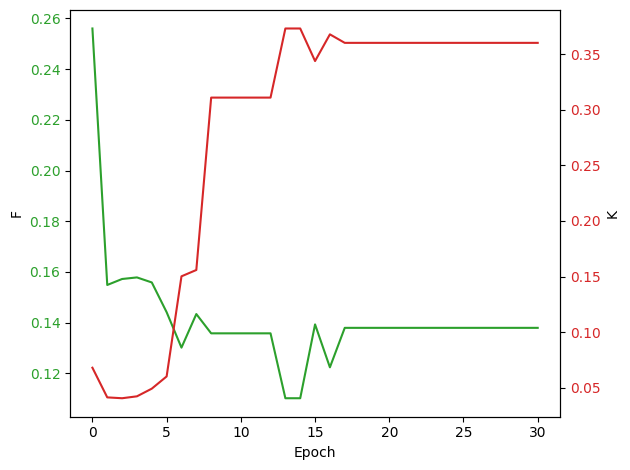
\includegraphics[width=.5\textwidth]{images/flower-params.png}}\hfill
            \subfloat[Control parameters]{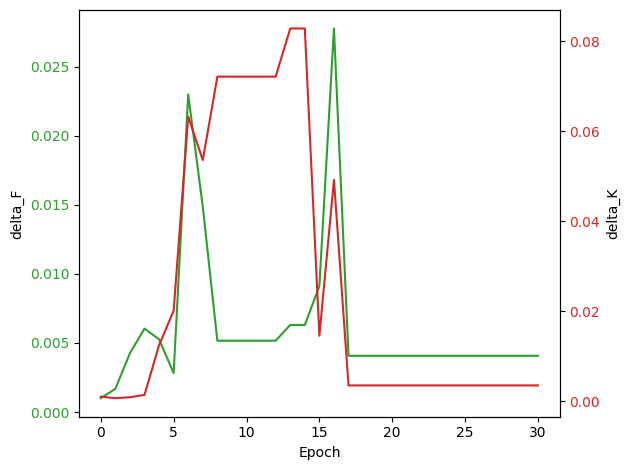
\includegraphics[width=.5\textwidth]{images/flower-derivs.png}}\hfill
            \caption{Evolution of \textit{flower} pattern using evolutionary strategy (population size = 20)}
\label{fig:flower-fail}
\end{figure}

Increasing the population size does not appear to resolve matters. Changing the discrete Laplacian operator to the alternative presented by Compeau\cite{compeau}
\[
  K= \begin{bmatrix}
    0.05 & 0.2 & 0.05\\
    0.2 & -1 & 0.2\\
    0.05 & 0.2 & 0.05
  \end{bmatrix}
\]
also appears to have no effect. These are shown in Figure~\ref{fig:more-fails}

\begin{figure}[!h]
\centering
            \subfloat[State paramaters for \textit{zebrafish} pattern (pop size = 50, Laplacian = nine-point stencil)]{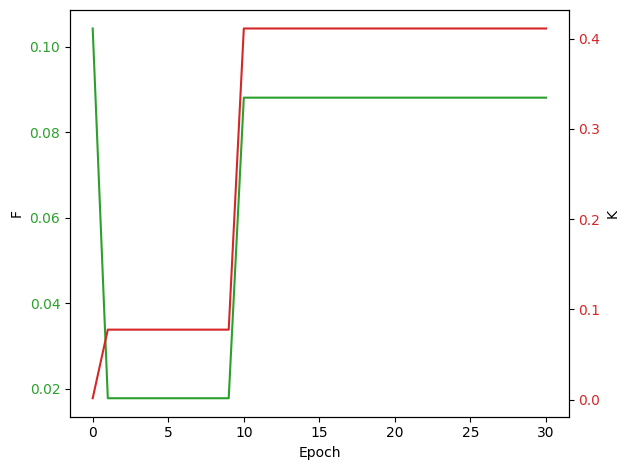
\includegraphics[width=.5\textwidth]{images/zebra-params.png}}\hfill
            \subfloat[State paramaters for \textit{soliton} pattern (population size = 25, Laplacian = Compeau operator)]{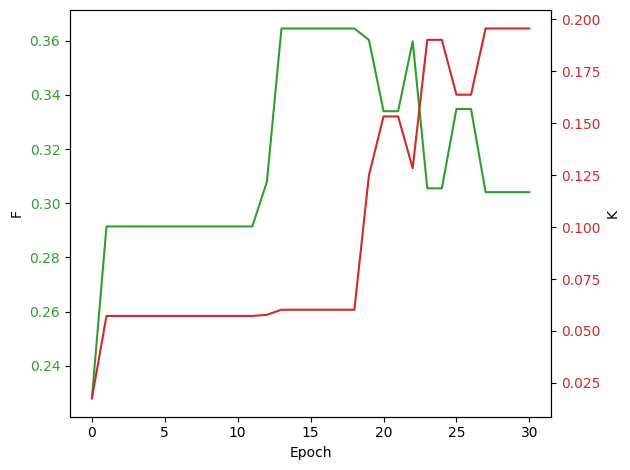
\includegraphics[width=.5\textwidth]{images/soliton-params.png}}\hfill
            \caption{Evolution of Gray-Scott models with different population sizes and Laplacian operators}
\label{fig:more-fails}
\end{figure}


The case for genetic algorithms is very similar. We tabulate the optima found and their distance from the target for each algorithm, chromosome initialisation method, initial condition, recombination operator, and mutation rate below. Figure~\ref{fig:big-fail-true} shows a simulation of the target pattern and figure~\ref{fig:big-fail-pred} shows a simulation of the local optimum that was discovered.\\

\begin{figure}
            \subfloat{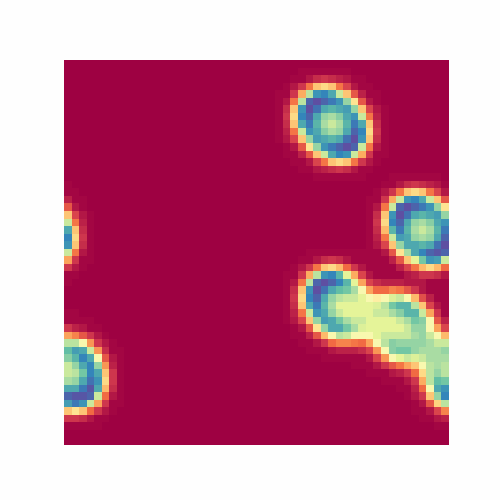
\includegraphics[width=.2\textwidth]{images/gray_scott/true/1.png}}\hfill
            \subfloat{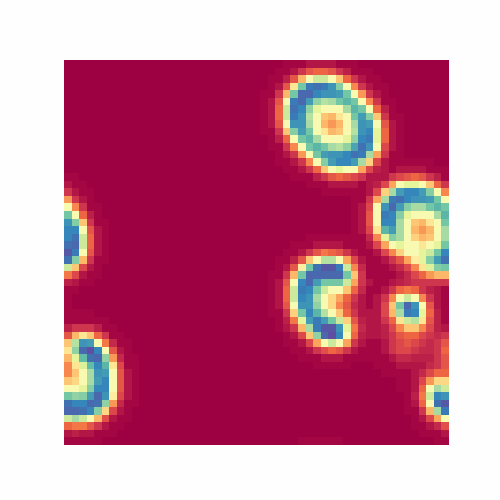
\includegraphics[width=.2\textwidth]{images/gray_scott/true/2.png}}\hfill
            \subfloat{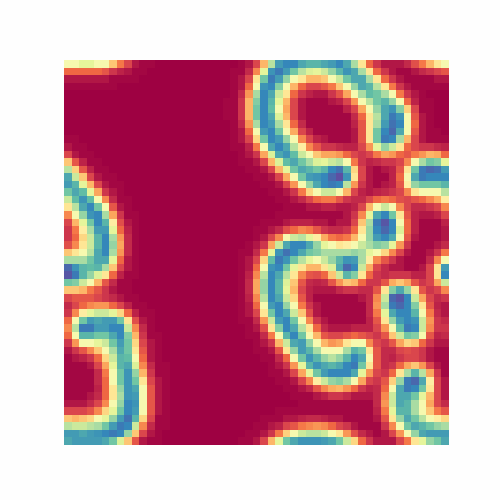
\includegraphics[width=.2\textwidth]{images/gray_scott/true/3.png}}\hfill
            \subfloat{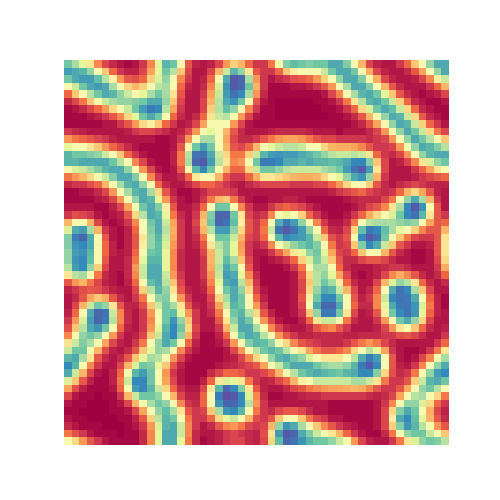
\includegraphics[width=.2\textwidth]{images/gray_scott/true/4.png}}\hfill
            \subfloat{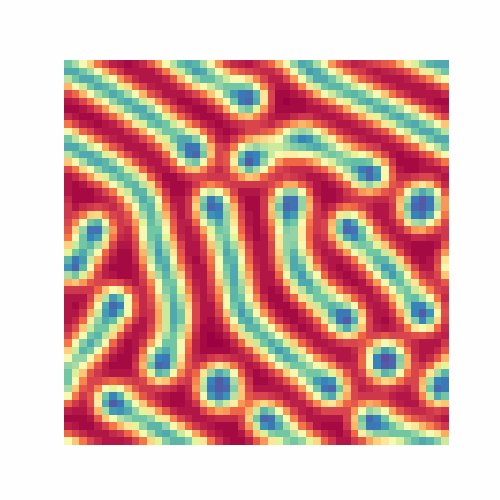
\includegraphics[width=.2\textwidth]{images/gray_scott/true/5.png}}\hfill
            \caption{Simulation of Gray-Scott target}
\label{fig:big-fail-true}
\end{figure}

\begin{figure}[!h]
\centering
            \subfloat{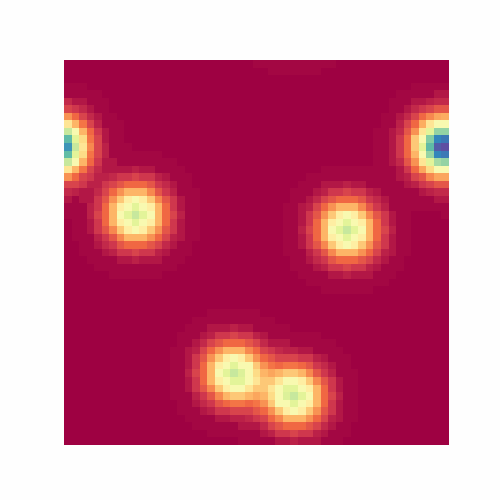
\includegraphics[width=.2\textwidth]{images/gray_scott/pred/1.png}}\hfill
            \subfloat{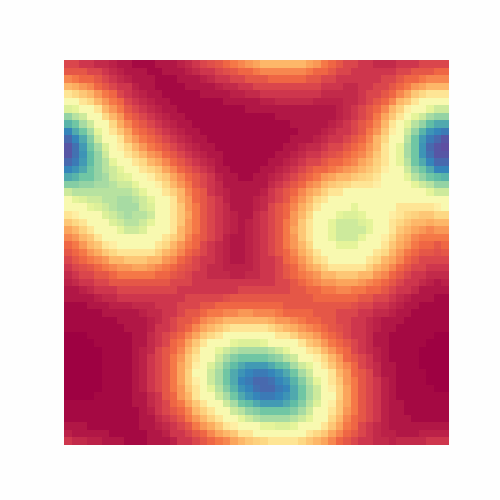
\includegraphics[width=.2\textwidth]{images/gray_scott/pred/2.png}}\hfill
            \subfloat{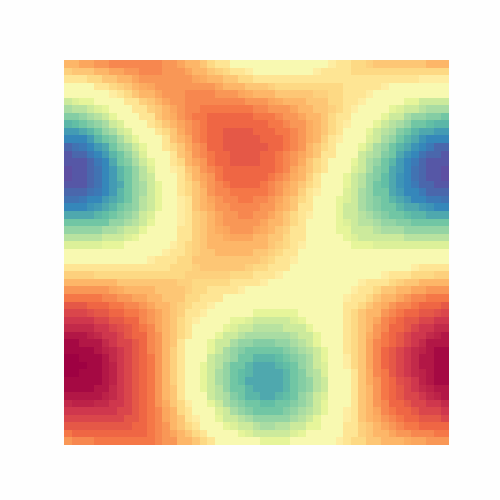
\includegraphics[width=.2\textwidth]{images/gray_scott/pred/3.png}}\hfill
            \subfloat{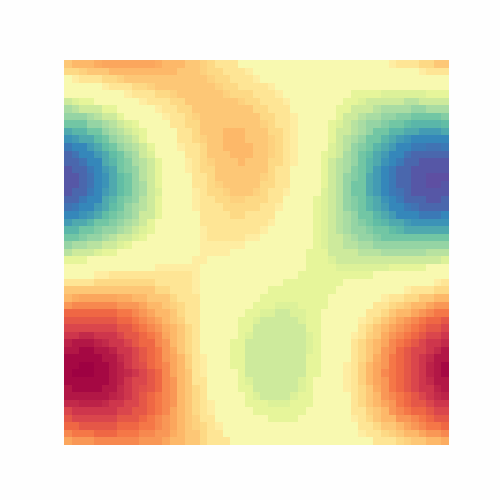
\includegraphics[width=.2\textwidth]{images/gray_scott/pred/4.png}}\hfill
            \subfloat{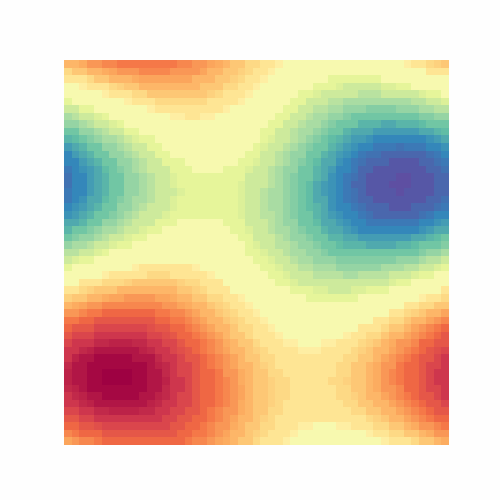
\includegraphics[width=.2\textwidth]{images/gray_scott/pred/5.png}}\hfill
            \caption{Simulation of Gray-Scott local optimum}
\label{fig:big-fail-pred}
\end{figure}

\todo{EXPERIMENT 2}: TODO - Populate this table with results from experiment 2

\begin{table}
    \centering\hfill
        \begin{tabular}{|c|c|c|c|c|c|c|}
            \hline
            Algorithm & Initialisation & Initial Condition & Recombination & Mutation Rate & Result & MSE \\
            \hline
            ES & Random  & Splatter & Plus & - & &  \\
            ES & Random  & Splatter & Comma & - & &  \\
            ES & Random  & Seed & Plus & - & &  \\
            ES & Random  & Seed & Comma & - & &  \\
            ES & Threshold  & Splatter & Plus & - & &  \\
            ES & Threshold  & Splatter & Comma & - & &  \\
            ES & Threshold  & Seed & Plus & - & &  \\
            ES & Threshold  & Seed & Comma & - & &  \\
            GA & Random  & Splatter & Plus & 0.001 & &  \\
            GA & Random  & Splatter & Comma & 0.001 & &  \\
            GA & Random  & Seed & Plus & 0.001 & &  \\
            GA & Random  & Seed & Comma & 0.001 & &  \\
            GA & Threshold  & Splatter & Plus & 0.001 & &  \\
            GA & Threshold  & Splatter & Comma & 0.001 & &  \\
            GA & Threshold  & Seed & Plus & 0.001 & &  \\
            GA & Threshold  & Seed & Comma & 0.001 & &  \\
            GA & Random  & Splatter & Plus & 0.01 & &  \\
            GA & Random  & Splatter & Comma & 0.01 & &  \\
            GA & Random  & Seed & Plus & 0.01 & &  \\
            GA & Random  & Seed & Comma & 0.01 & &  \\
            GA & Threshold  & Splatter & Plus & 0.01 & &  \\
            GA & Threshold  & Splatter & Comma & 0.01 & &  \\
            GA & Threshold  & Seed & Plus & 0.01 & &  \\
            GA & Threshold  & Seed & Comma & 0.01 & &  \\
            GA & Random  & Splatter & Plus & 0.1 & &  \\
            GA & Random  & Splatter & Comma & 0.1 & &  \\
            GA & Random  & Seed & Plus & 0.1 & &  \\
            GA & Random  & Seed & Comma & 0.1 & &  \\
            GA & Threshold  & Splatter & Plus & 0.1 & &  \\
            GA & Threshold  & Splatter & Comma & 0.1 & &  \\
            GA & Threshold  & Seed & Plus & 0.1 & &  \\
            GA & Threshold  & Seed & Comma & 0.1 & &  \\
            \hline
    \end{tabular}
\end{table}